\chapter{Referencial Teórico}
\label{cap:Referencial Teórico}

% figuras estão no subdiretório "figuras/" dentro deste capítulo
\graphicspath{\currfiledir/figuras/}


\section{AEs - Algoritmos Evolucionários}
\label{sec:aemos}


Um algoritmo evolucionário (AE) é uma técnica de busca, altamente paralela, inspirada na teoria da seleção natural e reprodução genética de Charles Darwin. De acordo com a teoria de Darwin, a seleção natural irá favorecer os indíviduos que forem mais aptos, dessa maneira, estes indíviduos tem uma maior probabilidade
de reprodução. Indivíduos com mais descendentes tem uma chance maior de perpetuarem seus códigos genéticos nas gerações futuras. O código genético é a identidade de cada indivíduo e é representado por cromossomos. Estes princípios são utilizados na implementação de algoritmos computacionais, que procuram por soluções melhores para um dado problema, evoluindo uma população 
de soluções codificadas em cromossomos artificais -- estruturas de dados utilizadas para representar soluções factíveis para um dado problema \cite{pacheco1999algoritmos}.

De maneira geral, problemas reais de otimização possuem múltiplos objetivos a serem minimizados/maximizados e estão presentes em muitas áreas do conhecimento.
Para otimizar problemas multiobjetivos dois ou mais objetivos são considerados, os quais geralmente são conflitantes. Para estes problemas é impossível encontrar uma
única solução ótima. Um conjunto de soluções é encontrado avaliando a dominância de Pareto \cite{pareto} entre as soluções. O objetivo principal é encontrar o conjunto  
de soluções que sejam não dominadas entre si. Uma solução domina outra, se e somente se, for melhor em pelos um dos objetivos, sem ser pior em qualquer outro.
Este conjunto de soluções constitui a fronteira de Pareto. Encontrar a fronteira real de Pareto é um problema NP-Completo \cite{fonseca2005tutorial}, dessa maneira,
o objetivo é encontrar uma boa aproximação da fronteira real.

Algoritmos Evolucionários Multi-Objetivos (AEMOs) são extensões de AEs para problemas multi-objetivos, os quais aplicam
conceitos da dominância de Pareto para criar diferentes estratégias para evoluir e manter a diversidade das soluções.
Nesta dissertação foram explorados dois AEMOs: NSGAII \cite{deb2002fast} and IBEA \cite{zitzler2004indicator}.
%=====================================================

\subsection{NSGAII - Non-dominated sorting Genetic Algorithm II}
\label{subsection:nsgaii}

O algoritmo \ref{alg:nsgaII} apresenta o pseudo código do NSGAII. O algoritmo recebe como parâmetro $N$ o tamanho da população e $T$ o número máximo 
de avaliações. O algoritmo inicia criando uma população com tamanho $N$ chamada $P_0$. A população $P_0$ é classificada de acordo com aptidão 
e a relação de não dominância. A população $P_0$ é submitida ao operador de seleção: torneio binário para selecionar duas soluções que serão utilizadas
para gerar descendentes. Operadores de cruzamento e mutação são aplicados na soluções selecionadas gerando duas soluções distintas descendentes. 
Ao fim do processo de reprodução, as soluções descendentes são avaliadas e adicionadas a população chamada $Q_0$.

Após esta estapa, $P_0$ e $Q_0$ são adicionadas em uma população auxiliar chamada $R$. Utilizando o conceito de não dominância, $R$ é ordenada 
criando fronteiras, onde cada solução da primeira fronteira não é dominada por nenhuma outra solução, já soluções da segunda fronteira são dominadas
apenas por soluções contidas na primeira fronteira, e assim por diante. Para cada fronteira, as soluções são avaliadas utilizando um mecanismo
de \textit{Crowding-Distance (CD)}. Soluções com maiores valores de CD irão ser adicionadas na população da próxima geração chamada $P_t$, no qual $t$ é a
avaliação corrente.

Após criar e preencher $P_t$ com as soluções não dominadas de todas as fronteiras, a população $P_t$ é avaliada e então passa para um novo
torneio binário e reprodução, dessa maneira, iniciando uma novo ciclo do algoritmo.

\begin{algorithm}[htb!]
	\begin{algorithmic}[1]
		\State{$N \gets$ Population Size}
		\State{$T \gets$ Max evaluations}
		\State{$P_0 \gets CreatePopulation(N);$}
		\State{$CalculateFitness(P_0);$}
		\State{$FastNonDominatedSort(P_0);$}
		\State{$Q_0 \gets 0$}
		\While{$Q_0 < N$}
		\State{$Parents \gets BinaryTournament(P_0);$}
		\State{$Offspring \gets CrossoverMutation(Parents);$}
		\State{$Q_0 \gets Offspring$}
		\EndWhile
		\State{$CalculateFitness(Q_0);$}
		\State{$t \gets 0$}
		\While{$t < T$}
		\State{$R_t \gets P_t \cup Q_t;$}
		\State{$Fronts \gets FastNonDominatedSort(R_t);$}
		\State{$P_{t+1} \gets 0$}
		\State{$i \gets 0$}
		\While{$P_{t+1} + Front_i  < N$}
		\State{$CrowdingDistanceAssignment(Front_i);$}
		\State{$P_{t+1} \gets P_{t+1} \cup Front_i$}
		\State{$i \gets i + 1$}
		\EndWhile
		\State{$CrowdingDistanceSort(Front_i);$}
		\State{$P_{t+1} \gets P_{t+1} \cup Front_i[1:(N -P_{t+1})]$}
		
		\State{$Parents \gets BinaryTournament(P_{t+1});$}
		\State{$Q_{t+1} \gets CrossoverMutation(Parents);$}
		\State{$t \gets t +1$}
		\EndWhile
		\State{\Return{$P \gets$ Set of non-dominated solutions.}}
	\end{algorithmic}
	\caption{NSGAII}
	\label{alg:nsgaII}
\end{algorithm}


%=====================================================

\subsection{IBEA (Indicator-Based Evolutionary Algorithm)}

No contexto de otimização multiobjetiva, otimizar consiste em tentar encontrar a fronteira com uma boa aproximação da fronteira real de Pareto. 
Entretanto, não existe uma definição geral para "uma boa aproximação". Consequentemente, indicadores de qualidade vem sendo utilizados
para avaliar a qualidade da aproximação de fronteiras. O indicador \textit{hypervolume} é um exemplo de indicador utilizado para avaliação e comparação 
das fronteiras.

No algoritmo IBEA, indicadores de qualidade são	utilizados para avaliar o conjunto de soluções não dominadas \cite{figueiredo2013algoritmo}.
Para utilizar o IBEA, é necessário definir qual indicador será utilizado para associar cada solução a um valor scalar. Um dos indicadores bastante utilizados é o \textit{hypervolume} por conta da sua capacidade de avaliar a convergência e a diversidade do espaço de busca ao mesmo \cite{ishibuchi2008evolutionary}.

\begin{equation} \label{eq:ibeaFitness}
F(x_i) = \sum_{x_j \in (P-x_i)} {-e^\frac{-I_{Hy}(x_j,x_i)}{k}}
\end{equation}

A equação de \textit{fitness} do IBEA é apresentada pela equação \ref{eq:ibeaFitness} e é utilizada para calcular a contribuição de uma dada solução
para o valor do indicador referente a população, onde $k$ é um fator escalar dependente do $I_{Hy}$, o qual representa o indicador de qualidade sendo utilizado. O valor $F(x_i)$ corresponde à perda de qualidade da aproximação, da fronteira real de Pareto, se a solução $x_i$ for removida da população \cite{figueiredo2013algoritmo}.


O Algoritmo \ref{alg:ibea} recebe como parametro o tamanho da população $N$, o número máximo de avaliações $T$ e o fator escalar $k$. O processo se inicia
criando uma população $P$ de tamanho $N$. Os seguintes passos irão se repetir até que o critério de parada seja atingido: um torneio binário 
para selecionar indivíduos, reprodução (cruzamento e mutação) dos indivíduos selecionados para gerar descendentes, adicionar os descedentes na população
auxiliar $\overline P$. Após a reprodução, a população $\overline P$ é unida com $P$. Enquanto o tamanho de $P$ exceder $N$, o pior indíviduo avaliado
pela equação \ref{eq:ibeaFitness} é removido da população $P$ e os indíviduos restantes são re-avaliados. Quando o algoritmo terminar irá retornar o conjunto
de soluções não dominadas é retornado.

\begin{algorithm}[htb!]
	\begin{algorithmic}[1]
		\State{$N \gets$ Population Size}
		\State{$\overline N \gets$ AuxiliaryPopulationSize}
		\State{$T \gets$ Max Evaluations}
		\State{$k \gets$ Scale factor of Fitness}
		
		\State{$P \gets$ CreatePopulation($N$);}
		\State{$\overline P \gets$ CreateEmptyAuxiliaryPopulation($\overline N$);}
		\State{$m \gets 0$}
		\State{CalculateFitness($P$);}
		
		\While{$m \ge T$ or other stop criterion is not reached}
		
		\State{$\overline P \gets$ BinaryTournament($P$);}
		\State{$\overline P \gets$ CrossoverMutation($\overline P$);}
		\State{$P \gets P \cup \overline P$}
		\State{$m \gets m+1$}
		
		\While{Size($P$) $> N$}
		\State{$x^* \gets$ WorstIndividualByFitness();}
		\State{RemoveFromPopulation($x^*$, $P$);}
		\State{CalculateFitness($P$);}
		\EndWhile
		
		\EndWhile
		\State{\Return{$P \gets$ Set of non-dominated solutions}}
		
	\end{algorithmic}
	\caption{IBEA}
	\label{alg:ibea}
\end{algorithm}

%\footnotetext[1]{\textit{Hypervolume}: Indicador de qualidade utilizado neste estudo \cite{zitzler1998multiobjective}, 
%	denotado como o "tamanho da área coberta do espaço de busca". Este indicador tem uma vantagen importante em relação aos outros \cite{zitzler2007hypervolume}:
%	1 - Sensitivo a qualquer tipo de melhoria na aproximação em relação a outro conjunto. 

\section{Hiper-Heurísticas }
\label{Hiper-Heuristicas}

Apesar do sucesso de métodos heurísticos e outros métodos de busca na tarefa de resolver problemas de busca computacional difíceis, ainda existem dificuldades em generalizar estes métodos para diferentes problemas ou até mesmo para diferentes instâncias de um mesmo problema. Esta dificuldade provém principalmente da necessidade de selecionar os parâmetros e configurações mais adequados dos algoritmos para um problema ou para uma dada instância de um problema. Também vale mencionar a pouca orientação na tarefa de definir estes parâmetros.  É neste contexto que surge uma questão: é possível automatizar o projeto e parametrização de métodos heurísticos para resolver problemas de busca computacional difíceis? \cite{burke2013hyper}. A ideia principal é desenvolver algoritmos que sejam mais genéricos do que as implementações de metodologias atuais \cite{burke2013hyper}. As principais abordagens já propostas para este desafio podem ser classificadas em duas categorias: configuração estática (\textit{offline}) e controle dinâmico (\textit{online}). Abaixo são apresentadas algumas abordagens já propostas na literatura:

\begin{itemize}
	\item Configuração Estática (Offline):
	\begin{itemize}
		\item Seleção de algoritmos;
		\item Portfólio de algoritmos;	
		\item Configuração de algoritmos;
		\item Ajuste de parâmetros;
		\item Hiper-Heurísticas.
	\end{itemize}
	\item Controle Dinâmico (Online):
	\begin{itemize}
		\item Seleção adaptativa de operadores (AOS);
		\item Controle de parâmetros;	
		\item Algoritmos meméticos adaptativos;
		\item Hiper-Heurísticas
	\end{itemize}
	
\end{itemize}


Esta seção tratará apenas de hiper-heurísticas e suas particularidades. Uma hiper-heurística pode ser vista como uma metodologia de alto nível, a qual seleciona ou cria heurísticas para resolver um dado problema ou instância de um problema. \cite{burke2013hyper}. O objetivo principal é tentar encontrar ou construir a heurística mais adequada para cada situação. As hiper-heurísticas diferem dos métodos padrão de busca, pois operam sobre o espaço de busca de heurísticas que por sua vez operam sobre o espaço de busca de um problema. Além disso, hiper-heurísticas são independentes do problema. Tradicionalmente frameworks hiper-heurísticos possuem dois níveis \cite{sabar2015automatic}: 

\textbf{Heurísticas de baixo nível}:  Um conjunto de heurísticas de baixo nível específicas. Estas heurísticas costumam diferir entre domínios de problemas. São exemplos: operadores de cruzamento, mutação e buscas locais. Em alguns casos, meta-heurísticas, dependendo da modelagem do \textit{framework} hiper-heurístico, também podem assumir o papel de heurísticas de baixo nível. 

\textbf{Heurísticas de alto nível}: Geralmente consistem em dois componentes: mecanismo de seleção, que gerencia quais heurísticas de baixo nível devem ser aplicadas durante a busca; um critério de aceitação, que tem a responsabilidade de decidir se irá aceitar ou não uma solução gerada, a partir da aplicação de uma heurística de baixo nível. A responsabilidade do mecanismo de seleção é selecionar, de um \textit{pool} de heurísticas de baixo nível, a heurística que for mais adequada naquele momento. Geralmente, a escolha da heurística de baixo nível é crucial para uma boa exploração do espaço de busca, evitando que a busca fique confinada em uma região específica \cite{sabar2015automatic}. O objetivo do critério de aceitação é auxiliar o processo de busca a evitar mínimos locais assim como explorar diferentes regiões através do aceite ou rejeição de soluções geradas \cite{chakhlevitch2008hyperheuristics}. Espera-se que um bom critério de aceitação deva atingir um bom equilíbrio entre aceitar soluções melhores assim, como soluções diversificadas caso a busca esteja presa em um mínimo local \cite{sabar2015automatic}. Ambos os componentes devem ser independentes de conhecimento sobre o problema.

A Imagem \ref{img:hiperheuristico} apresenta um diagrama exemplificando os níveis de um \textit{framework} hiper-heurístico e suas características. Note que entre os níveis (alto e baixo) existe uma barreira de domínio, ou seja, apenas as heurísticas de baixo nível são dependentes de conhecimento do problema ou instância enquanto as heurísticas de alto nível não são dependentes do problema. 

\begin{figure}[!htb]
	\centering
	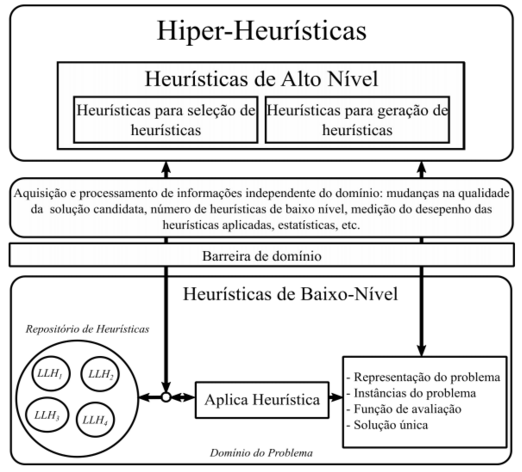
\includegraphics{Imagens/HiperHeuristicas.png}
	\caption{Framework Geral Hiper-Heurístico. Adaptado de \cite{sabar2015automatic}}
	\label{img:hiperheuristico}
\end{figure}


Como cada instância ou problema possui um espaço de busca com diferentes características, os componentes da heurística de alto nível têm um grande impacto no desempenho de um \textit{framework} hiper-heurístico. Esta é uma das razões de existir um grande interesse de pesquisa em desenvolver  novos mecanismos de seleção, assim como diferentes critérios de aceitação \cite{burke2013hyper}. Um bom mecanismo de seleção deve selecionar a heurística mais adequada em um dado momento, para guiar a busca para regiões promissoras do espaço de busca. 
Ao utilizar hiper-heurísticas, espera-se encontrar o método correto ou a sequência de heurísticas que mais se adequam a um problema ou instância em vez de tentar resolver o problema diretamente. Entretanto, um importante objetivo é desenvolver métodos genéricos, que têm  potencial em produzir soluções com uma qualidade aceitável, utilizando um conjunto de heurísticas de baixo nível com fácil implementação. As hiper-heurísticas podem ser classificadas de diversas maneiras. A Figura \ref{img:classificacaoHiperHeuristicas} apresenta as possíveis classificações descritas na literatura. 

\begin{figure}[!htb]
	\centering
	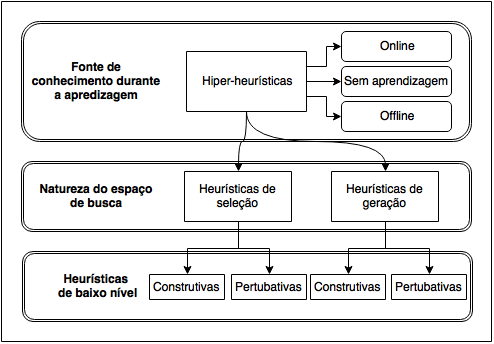
\includegraphics[scale=0.8]{Imagens/ClassificacaoHiperHeuristica.png}
	\caption{Classificação Hiper-heurísticas. Adaptado de \cite{sabar2015automatic}}
	\label{img:classificacaoHiperHeuristicas}
\end{figure}

A primeira classificação de hiper-heurísticas é baseada na sua fonte de conhecimento durante a busca: \textit{Online} é quando a hiper-heurística toma decisões de maneira instantânea, baseando-se em métricas durante sua execução, não necessitando de treinamento prévio. \textit{Offline} necessita de treinamento prévio; estes \textit{frameworks}  tomam suas decisões baseados no que foi aprendido apenas durante o treinamento, sem atualização deste conhecimento. Os \textit{frameworks} classificados como \textit{No-Learning} não possuem nenhuma forma de aprendizagem. Outra classificação considera a forma como as heurísticas de baixo nível operam sobre as soluções do problema. As heurísticas ditas perturbativas realizam pequenas perturbações nas soluções gerando novas soluções. Já heurísticas construtivas criam soluções do zero passo a passo e normalmente avaliam cada etapa da construção para obter \textit{feedback} sobre o seu desempenho. Uma última  classificação, mas não menos importante, divide as hiper-heurísticas de acordo com a  natureza do seu espaço de busca. As hiper-heurísticas de seleção selecionam sequências de heurísticas a serem aplicadas para resolver um dado problema ou instância. Já as hiper-heurísticas de geração operam gerando novas heurísticas com objetivo de resolver um problema ou instância.


\subsection{Hiper-heurísticas de Geração}
\label{Hiper-Heuristicas-Geraçao}

Estas hiper-Heurísticas geram novas heurísticas combinando componentes de heurísticas existentes. Geralmente se utiliza programação genética (GP), ou alguma vertente de GP, como evolução gramatical \cite{ryan1998grammatical} ou programação gênica \cite{ferreira2006gene}, como hiper-heurística para gerar heurísticas. A próxima sub-seção irá introduzir o conhecimento necessário para a compreensão da programação genética, assim como irá introduzir evolução gramatical, que se trata de um tipo de programação genética e que será utilizada nesta proposta.

\section{Programação Genética (PG)}
\label{subsection:PG}

Programação Genética \cite{burke2009exploring} é um ramo da síntese de programas que utiliza ideias oriundas da teoria da evolução natural para produzir programas. Os principais componentes da computação evolucionária são herança (cruzamento/reprodução), seleção e variação (mutação). A herança significa que os descendentes  têm alguma semelhança com seus pais, pois quase todo material genético vem dos pais. A seleção trata de escolher quais pais irão se reproduzir para gerar novos descendentes; pais com maior aptidão tendem a ter maior probabilidade de serem selecionados. Esta pressão de seleção define quais indivíduos estão mais aptos que outros. Variação realiza pequenas alterações em um descendente a fim de criar novo material genético neste indivíduo e que não estava presente em nenhum dos indivíduos que o geraram. Computação evolutiva pode ser pensada como a interação destes três componentes. 
Uma população aleatória de programas de computador é gerada, e os operadores geneticamente inspirados (cruzamento e mutação) são repetidamente aplicados com objetivo de produzir novos programas de computador. Estes programas são avaliados utilizando uma função de \textit{fitness} (normalmente dependente do desempenho obtido pela aplicação do programa em um problema), que determina quais destes programas são mais suscetíveis a sobreviver para gerações futuras. Os programas com maior aptidão tem mais chances de serem selecionados para o cruzamento e perpetuarem parte de seus códigos genéticos durante o processo evolutivo. 
Programação genética é um método de geração de programas sintaticamente válidos e a função de \textit{fitness} é utilizada para decidir quais programas são mais adequados para o problema.
Na programação genética, os programas que compõem a população são tradicionalmente representados utilizando estruturas de árvore. Existem outras estruturas que podem ser evoluídas, por exemplo: sequências lineares de instruções ou gramáticas. Nesta proposta será utilizada uma representação gramatical linear que será explicada na Seção \ref{subsubsection:EvolucaoGramatical}.

\section{Evolução Gramatical (EG)}
\label{subsubsection:EvolucaoGramatical}

Evolução gramatical é uma técnica relativamente nova de computação evolutiva, proposta por Ryan et al. \cite{ryan1998grammatical}. Trata-se de um tipo de programação genética. Assim como na programação genética, o principal objetivo é encontrar um programa executável ou trecho de um programa, que obtenha um bom valor de \textit{fitness} para o problema em questão. Na maioria dos trabalhos publicados de programação genética, expressões que representam estruturas de árvore são manipuladas, enquanto na evolução gramatical os operadores genéticos são aplicados em vetores de inteiros que posteriormente são mapeados para um programa (ou trecho de programa) através de uma gramática específica. Um dos benefícios de EG é que este mapeamento generaliza a aplicação para diferentes linguagens de programação. \cite{ryan1998grammatical} propõem uma técnica para gerar programas ou fragmentos de programas para qualquer linguagem de programação utilizando definições BNF. A técnica pode ser utilizada para evoluir programas por um processo evolutivo. A evolução gramatical adota um mecanismo de mapeamento entre o genótipo (indivíduos codificados em um vetor de inteiros) e o fenótipo (programas gerados para resolver algum problema). 
A notação \textit{Backus Naur Form} (BNF) é a notação utilizada para expressar a gramática de uma linguagem na forma de regras de produção. Uma gramática BNF consiste em um conjunto de terminais, os quais são itens que podem aparecer na linguagem, por exemplo: +, -, *, / etc e não terminais, que podem ser expandidos em um ou mais terminais e não terminais. Uma gramática pode ser expressada como uma tupla ${N,T,P,S}$, onde $N$ é o conjunto de não terminais, $T$ o conjunto de terminais, P um conjunto de regras de produção que mapeia os elementos $N$ para $T$; e, por último, $S$, um símbolo de início e que está contido em $N$.

\begin{center}
	
	$ N = {\langle expr \rangle, \langle op \rangle, \langle pre-op \rangle}$
	
	$ T = {Sin,Cos,Tan,Log,+,-,/,*,X} $
	
	$ S = \langle expr \rangle $
	
\end{center}

\noindent
E $P$ pode ser representada como:

\begin{Grammar}
	\begin{grammar}
		
		
		<expr> ::=  <expr> <op> <expr> \hspace{10cm} (0) 
		\alt (<expr> <op> <expr>) \hspace{9.7cm} (1)  
		\alt <pre-op> (<expr>) \hspace{10.15cm} (2) \alt <var> \hspace{12.1cm} (3) \\\
		
		<op> ::=  + \hspace{12.7cm} (0)   \alt - \hspace{12.8cm} (1)  \alt  /  \hspace{12.85cm} (2) \alt * \hspace{12.75cm} (3) \\
		
		<pre-op> ::= Sin  \hspace{12.4cm} (0) \alt Cos
		\hspace{12.3cm} (1) \alt Tan  \hspace{12.35cm} (2)
		
		<var> ::= X  \hspace{12.6cm} (0)
		
		
	\end{grammar}
	
	\caption{Gramática exemplo para demonstrar como decodificar vetores de inteiros em programas de computador.}
	\label{gram:gramatica}
\end{Grammar}


\begin{table}[htb]
	\centering
	\caption{\textit{Regras de produção} e o número de escolhas para cada uma.}
	\label{tab:productionRules}
	\begin{tabular}{|l|l|}
		\hline
		Regra de produção & Número de escolhas \\ \hline
		$\langle expr \rangle$                        & 4       \\ \hline
		$\langle op \rangle$                         & 4       \\ \hline
		$\langle pre-op \rangle$                         & 3       \\ \hline
		$\langle var \rangle$                          & 1       \\ \hline
	\end{tabular}
\end{table}


Ryan et al. \cite{ryan1998grammatical}  propôs o uso de um algoritmo genético (AG) para controlar quais escolhas devem ser feitas, permitindo dessa maneira que o AG controle quais regras de produção serão utilizadas. Um indivíduo (cromossomo) consiste em um vetor de tamanho variável de valores inteiros que representa o genótipo. Para fins de compreensão o processo de mapeamento de um cromossomo será demonstrado utilizando a \autoref{gram:gramatica} apresentada anteriormente nesta seção. O Algoritmo \ref{alg:pseudocodigogrammar} apresenta o \textit{template} geral dos programas gerados pela \autoref{gram:gramatica}. A expressão $\langle expr \rangle$ apresentada na linha 2 do Algoritmo \ref{alg:pseudocodigogrammar} é substituída por expressões matemáticas que estão codificadas pelos cromossomos (vetores de inteiros). 

\begin{algorithm}
	\caption{\textit{Template} geral dos algoritmos gerados}
	\label{alg:pseudocodigogrammar}
	float symb(float x) { \\
		a = $\langle expr \rangle$;   \\
		return a;  \\
	}	
\end{algorithm}

\noindent
Suponha o seguinte vetor de inteiros:

\begin{center}
	$ [220, 203, 17, 6, 108, 215, 104, 30] $
\end{center}


Este vetor será utilizado para mapear o cromossomo (genótipo) em um trecho de programa (fenótipo) utilizando a gramática BNF. 
%A expressão não terminal $ \langle expr \rangle$ no algoritmo \ref{alg:pseudocodigogrammar} será preenchida por um trecho de código que será mapeado a partir do cromossomo apresentado. Os passos do mapeamento serão descritos a seguir.%
A tabela \autoref{tab:productionRules} resume o número de escolhas associada à cada regra de produção da \autoref{gram:gramatica}. Existem 4 opções de regras de produção que podem ser selecionadas para a expressão $ \langle expr \rangle$. Para decidir qual será selecionada, o primeiro valor no cromossomo deve ser utilizado. Sendo que o valor é 220. Devemos realizar o módulo deste valor pelo número de escolhas, neste caso 4. Portanto, 220 MOD 4 = 0, o que significa selecionar a primeira opção: $\langle expr \rangle \langle op \rangle \langle expr \rangle$.

Note que a primeira expressão é novamente $ \langle expr \rangle$ e da mesma maneira devemos obter o próximo valor de inteiro e realizar o módulo. O próximo valor inteiro é 203; realizando o modulo de 4, resulta em 3, que portanto seleciona a quarta opção: $ \langle var \rangle$. Substituindo na expressão anterior, obtemos: $ \langle var \rangle \langle op \rangle \langle expr \rangle$

Nenhuma escolha é necessária para a expressão $ \langle var \rangle$, pois existe apenas uma opção $X$. A expressão pode ser reescrita da seguinte maneira: $X \langle op \rangle \langle expr \rangle$

Neste momento é necessário decodificar a expressão não terminal $\langle op \rangle$. Obtendo o próximo valor inteiro do cromossomo, temos 17 e para o $ \langle op \rangle$ temos 4 opções $(+ | - | / | *)$. O resultado de 17 MOD 4  é igual a 1, que significa selecionar:  $-$. Substituindo na expressão, temos: $X  -  \langle expr \rangle$


Novamente é necessário fazer uma nova escolha para resolver a expressão não terminal $\langle expr \rangle$. O próximo valor do cromossomo é 6 e novamente existem 4 opções. Realizando o modulo 6 MOD 4, obtém-se 2, que seleciona $ \langle pre-op \rangle ( \langle expr \rangle)$. Atualizando a expressão, obtemos: $X - \langle pre-op \rangle (\langle expr \rangle)$

Resolvendo a expressão $ \langle pre-op \rangle$, obtemos 108 MOD 4 = 0 que por sua vez seleciona a primeira expressão  terminal $Sin$. Atualizando a expressão, obtemos: $X - Sin (\langle expr \rangle)$

Expandindo $ \langle expr \rangle$, obtemos 215 MOD 4 = 3, que seleciona a expressão não terminal $ \langle var \rangle$. Já que para a expressão $ \langle var \rangle$ existe apenas uma opção, nenhuma escolha é necessária e a expressão final decodificada (fenótipo) é: $X - Sin (X)$

Note que nem todos os genes do cromossomo foram necessários para obter o fenótipo. Nos casos em que isto ocorre, os genes que não forem utilizados são desconsiderados. Além disso, pode ocorrer que um cromossomo não tenha genes suficientes para mapear um programa. Neste caso a estratégia é reutilizar os genes do cromossomo a partir do primeiro gene. 

Operadores genéticos tradicionais (cruzamento e mutação) também são utilizados na EG. Além dos operadores tradicionais outros dois operadores \textit{Prune} e \textit{Duplicate} são peculiares à EG e serão descritos em seguida:

\begin{itemize}
	\item \textit{Duplicate}: Este operador (dada uma probabilidade) realiza a cópia de  alguns genes. Os genes duplicados são adicionados após a última posição do cromossomo. O número de genes a serem duplicados é selecionado de maneira aleatória. A motivação por trás deste operador é que ao duplicar genes ocorre um aumento da presença de genes que são potencialmente bons, pois pertencem a um indivíduo com boa aptidão selecionado pelo operador de seleção.
	\item \textit{Prune} : Este operador leva em consideração que nem sempre todos os genes, de um cromossomo, são utilizados para decodificar um programa. Dessa maneira (dada uma probabilidade) realiza o truncamento de  cromossomos. O objetivo é diminuir a probabilidade que o operador de cruzamento opere em regiões dos cromossomos que não sejam utilizadas realmente.
\end{itemize}


O Algoritmo \ref{alg:GE} apresenta o pseudocódigo da evolução gramatical (EG). Note que o pseudocódigo é muito similar a um algoritmo genético simples. Nas linhas 3 e 4 ocorre a inicialização da população e o mapeamento para programas utilizando a gramática que foi provida como entrada. Em seguida, na linha 5 ocorre a execução dos programas e na linha 6 acontece a avaliação dos indivíduos da população, baseando-se na saída obtida pelos respectivos programas. Dentro do laço principal, apresentado na linha 7, podemos observar o processo de seleção dos indivíduos pais na linha 8 e na linha 9 o processo de cruzamento destes indivíduos. Nas linhas 10 e 11 ocorre a aplicação dos operadores \textit{Prune} e \textit{Duplicate} respectivamente e na linha 12 podemos observar a aplicação do operador de mutação. Em seguida, nas linhas 13,14 e 15 ocorre o mapeamento dos indivíduos descendentes para programas, execução dos programas e finalmente a atribuição de \textit{fitness} para os descendentes. Por fim, na linha 16 do laço principal, ocorre a substituição dos descendentes na população. 


%exceto pela aplicação dos operadores \textit{Duplicate} e \textit{Prune} (linhas 10 e 11 do Algoritmo  \ref{alg:GE}) e o processo de decodificação e execução dos programas descendentes (linhas 13 e 14 do Algoritmo \ref{alg:GE}).

\begin{algorithm}[htb!]
	%\fontsize{8pt}{10pt}\selectfont
	
	
	\begin{algorithmic}[1]
		\State{$AG  \gets$ Arquivo da gramática;}
		\State{$população \gets$ Inicialização a população;}
		\State{$programas \gets$ Mapeia $população$ para programas utilizando $AG$;}
		\State {Executa os $programas$;}
		\State {Atribui valor de \textit{fitness} para as soluções  of $população$ de acordo com a saída obtida pelos respectivos programas decodificados;}
%		\While{Condição de parada não atingida}
		\While{Condição de parada não atingida}
			\State {$pais \gets $ Seleção de indivíduos para cruzamento;}
			\State {$descendentes \gets$ Cruzamento $pais$;}
			\State {Aplica o operator \text{Prune} nas soluções $descendentes$;}
			\State {Aplica o operador \textit{Duplicate} nas soluções $descendentes$;}
			\State {Aplica o operador de mutação nas soluções $descendentes$;}
			\State {$programas \gets$ Mapeia $descendentes$ para programas utilizando $AG$;}
			\State {Executa $programas$;}
			\State {Atribui valor \textit{fitness} para as soluções $descendentes$ de acordo com a saída obtida pelos respectivos programas decodificados;}
			\State 	{$população \gets$ Realiza substituição;}
		\EndWhile \\
		\Return{Melhor programa da $população$;}
			
			
		
	\end{algorithmic}
	\caption{Pseudocódigo da evolução gramatical}
	\label{alg:GE}
\end{algorithm}


\section{Programação Genética como Hiper-Heurística de Geração de Heurísticas}
\label{subsubsection:PGasHH}

Nesta seção serão apresentadas questões relativas ao uso de EG como mecanismo de geração de heurísticas  \cite{burke2009exploring} descrevem que muitos autores mencionam a melhor adequação de programação genética, em relação a outras técnicas de aprendizagem de máquina, para gerar heurísticas de maneira automática. \cite{burke2009exploring} também apontam algumas vantagens desta técnica:

\begin{itemize}
	\item PG utiliza cromossomos de tamanho variável. Geralmente, não se sabe um tamanho ótimo para representar heurísticas de um dado domínio de problema.
	\item PG produz estruturas de dados executáveis. E heurísticas são tipicamente expressadas como programas ou algoritmos.
	\item Facilidade em identificar boas características do domínio do problema, afim de definir o conjunto terminal que será utilizado pela PG.
	\item Heurísticas desenvolvidas por humanos podem facilmente ser expressadas na mesma linguagem utilizada para criar o espaço de busca da PG. O conjunto de funções, relevante para o problema pode ser determinado facilmente. E adicionalmente PG pode ser suplementada com uma gramática específica.
\end{itemize}

Todas estas vantagens descritas por \cite{burke2009exploring} também são consideradas ao utilizar EG, visto que se trata de uma extensão de programação genética e possui as mesmas características (cromossomo de tamanho variável, produz estruturas executáveis, etc). \cite{burke2009exploring} também mencionam desvantagens, por exemplo: a cada execução da programação genética é encontrada uma melhor heurística que, por se tratar de uma técnica estocástica, os resultados podem ser distintos em diferentes execuções. Portanto, se fazem necessárias múltiplas execuções a fim de se obter um melhor conhecimento da qualidade das heurísticas que podem ser produzidas. Outra desvantagem é referente à configuração de parâmetros, que normalmente é encontrada via tentativa e erro.

\subsubsection{Abordagem Básica}

\cite{burke2009exploring} descrevem uma abordagem básica para aplicar programação genética para gerar heurísticas:

\begin{enumerate}
	\item Examinar as heurísticas existentes: Avaliar se as heurísticas já propostas para um dado problema podem ser descritas em um \textit{framework} comum. Estas heurísticas podem ter sido criadas por humanos ou até mesmo concebidas via outras técnicas de aprendizagem. Este passo não é trivial, pois envolve o entendimento de um número diverso de heurísticas existentes, que podem operar de diferentes maneiras. Geralmente heurísticas desenvolvidas por humanos são produtos de anos de pesquisa, e portanto, uma boa compreensão das heurísticas existentes pode ser um trabalho difícil. 
	\item Um framework que utilizará as heurísticas: neste momento a preocupação é em como as heurísticas serão aplicadas para um dado problema. Em geral, os frameworks tendem a ser bem diferentes dependendo do domínio do problema. 
	\item Definição do conjunto terminal: neste passo a preocupação refere-se a variáveis que expressem o estado do problema. Estas variáveis irão compor os terminais da programação genética/evolução gramatical. Outros terminais também podem ser utilizados. Particularmente, constantes aleatórias podem ser úteis.
	\item Definição do conjunto de funções: é necessário definir como as variáveis estarão relacionadas ou combinadas entre si. Estes relacionamentos irão compor o conjunto de funções da programação genética/evolução gramatical. 
	\item Identificar uma função de \textit{fitness}: uma função de \textit{fitness} precisa ser identificada para o problema. Geralmente, uma função simples de aptidão não irá avaliar bem os cromossomos. Introduzir alguns parâmetros pode ajudar a encontrar uma mais adequada.
	\item Executar o framework: geralmente ao executar pela primeira vez um framework hiper-heurístico com programação genética, não serão produzidos bons resultados, devido à escolha dos parâmetros. Isto é observado especialmente em casos que o pesquisador é iniciante. Portanto, é essencial que as definições de parâmetros sejam cuidadosamente investigadas.
\end{enumerate}




\section{Considerações Finais}
\label{ReferencialTeorico:Conclusão}


Neste capítulo foram apresentados alguns conceitos que permeiam a área de estudo otimização multi objetiva e sobre hiper-heurísticas. Inicialmente, uma contextualização sobre AEs foi fornecida em seguida os AEMOs foram introduzidos. Nesta dissertação foram utilizados os algoritmos NSGAII e IBEA os quais também foram apresentados. Também foi discutido sobre \textit{frameworks} hiper-heurísticos,  os seus níveis (alto e baixo) e as classificações encontradas na literatura.  Foram discutidas algumas estratégias para hiper-heurísticas de seleção e geração. As hiper-heurísticas de geração foram mais detalhadas, pois esta proposta visa o projeto  automático de heurísticas de alto nível. Foram apresentados os conceitos de PG e sua extensão EG, por se tratarem de estratégias comumente utilizadas para o projeto de hiper-heurísticas de geração de heurísticas. Também foram discutidas algumas vantagens e desvantagens referentes ao uso de PG para geração de heurísticas, além de demonstrar que a EG possui as mesmas características da PG, pois se trata de uma extensão que utiliza uma gramática para gerar os programas. O funcionamento geral da EG foi demonstrado utilizando uma gramática exemplo e um vetor de inteiros e, por fim, o pseudocódigo da evolução gramatical foi apresentado. 

O Capítulo \ref{cap:Trabalhos Relacionados} apresenta os trabalhos relacionados e o Capítulo \ref{cap:Metodologia} apresentará as abordagens propostas nesta dissertação. Já o Capítulo \ref{cap:experimentos} apresentá os experimentos realizados para cada abordagem e uma discussão sobre os resultados é realizada. E por fim o Capítulo \ref{cap:conclusao} apresentá a conclusão final desta dissertação.



